\begin{figure}
  \centering
  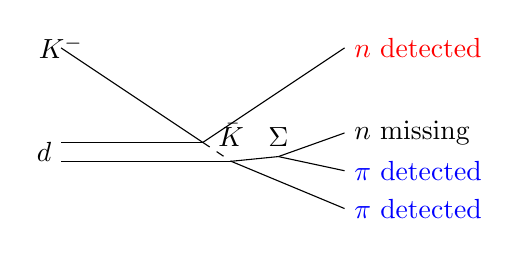
\begin{tikzpicture}[scale=1.2]
    \draw (-1.5,    1) node {$K^-$}--(0,    0);
    \draw (-1.5,    0)--(0,    0);
    \draw (-1.5, -0.2)--(0.3, -0.2);
    \node (d) at (-1.5, -0.1) [left] {$d$};

    \draw (0, 0) -- (0.3, -0.2) [dashed];
    \node (barK) at (0.3, -0.15) [above] {$\bar{K}$};

    \draw ( 1.5,  1.0) node [right] {\textcolor{red}{$n$ detected}}      -- (0,    0);
    
    \draw ( 1.5,  -0.7) node [right] {\textcolor{blue}{$\pi$ detected}} -- (0.3, -0.2);
    
    \draw ( 0.8,  -0.15) node [above] {$\Sigma$}    -- (0.3, -0.2);
    \draw ( 0.8,  -0.15) -- (1.5, 0.1) node [right] {$n$ missing};
    \draw ( 0.8,  -0.15) -- (1.5, -0.3) node [right] {\textcolor{blue}{$\pi$ detected}};    
  \end{tikzpicture}\\
  (a)
  
  \begin{tabular}{cc}
    \begin{minipage}{0.5\hsize}
      \centering
      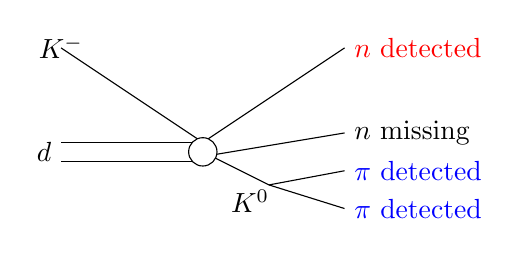
\begin{tikzpicture}[scale=1.2]
        \draw (-1.5,    1) node {$K^-$}--(0,    0);
        \draw (-1.5,    0)--(0,    0);
        \draw (-1.5, -0.2)--(0, -0.2);
        \node (d) at (-1.5, -0.1) [left] {$d$};
        
        \draw ( 1.5,  1.0) node [right] {\textcolor{red}{$n$ detected}}      -- (0,    0);

        
        \node (K0) at (0.5, -0.4) [below] {$K^0$};
        \draw (0, -0.1) -- (0.7, -0.45);
        
        \draw ( 0.0,  -0.15) -- (1.5, 0.1) node [right] {$n$ missing};
        \draw ( 0.7,  -0.45) -- (1.5, -0.3) node [right] {\textcolor{blue}{$\pi$ detected}};
        \draw (1.5,  -0.7) node [right] {\textcolor{blue}{$\pi$ detected}} -- (0.7, -0.45);
        
        \filldraw [fill=white] (0, -0.1) circle [radius=0.15];
      \end{tikzpicture}\\
      (b)
    \end{minipage}
    \begin{minipage}{0.5\hsize}
      \centering
      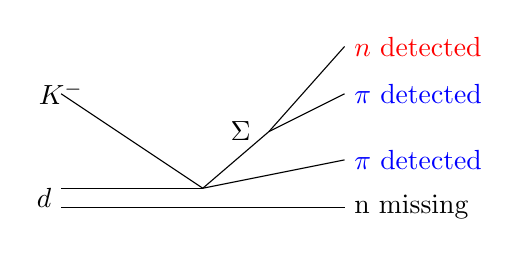
\begin{tikzpicture}[scale=1.2]
        \draw (-1.5,    1) node {$K^-$}--(0,    0);
        \draw (-1.5,    0)--(0,    0);
        \draw (-1.5, -0.2)--(0.3, -0.2);
        \node (d) at (-1.5, -0.1) [left] {$d$};

        \draw ( 1.5,  -0.2) node [right] {n missing} -- (0.3, -0.2);
        \draw ( 1.5,  0.3) node [right] {\textcolor{blue}{$\pi$ detected}}      -- (0,    0);

        \node (barK) at (0.4, 0.4) [above] {$\Sigma$};
        \draw ( 0.7,  0.6) -- (0.0, 0.0);
                
        \draw ( 0.7,  0.6) -- (1.5, 1.5) node [right] {\textcolor{red}{$n$ detected}};
        \draw ( 0.7,  0.6) -- (1.5, 1.0) node [right] {\textcolor{blue}{$\pi$ detected}};    
      \end{tikzpicture}\\
      (c)
    \end{minipage}
  \end{tabular}
  \label{fig:kd_npipin_type}
\end{figure}
